\subsection{Laboratory : Photoreceptors }

In this lab we will compare the source-follower (SF) photoreceptor with the unity-gain active transimpendance feedback (TI) photoreceptor.

\subsubsection{Static DC responses}
First, we study the response of these two circuits to a static input photocurrent.
These two circuits have symmetrical responses                                at the output voltage. To put it simply, with less light the SF photoreceptor outputs a bigger voltage and viceversa for the TI photoreceptor. 

\begin{figure}[H]
    \centering
    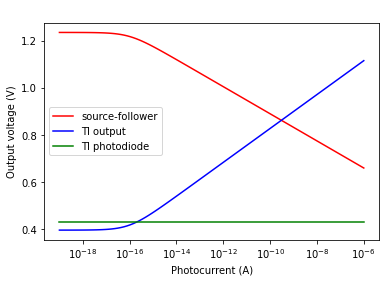
\includegraphics[width=0.75\linewidth]{Figures/photo_output.png}
    \caption{DC Photoreceptors responses}
    \label{fig:basalandcerebellum}
\end{figure}

\subsubsection{Large signal transient response}

Next, we compute the large signal transient response. Similarly to the lab on linear systems, we need to compute the ordinary differential equation for both photo receptors. 

Less photocurrent translates to more output voltage in the SF photoreceptor. In the time domain with a large input step, SF response is almost symmetrical to the current, whereas TI response behaves similar to a Follower Integrator.

\begin{figure}[H]
    \centering
    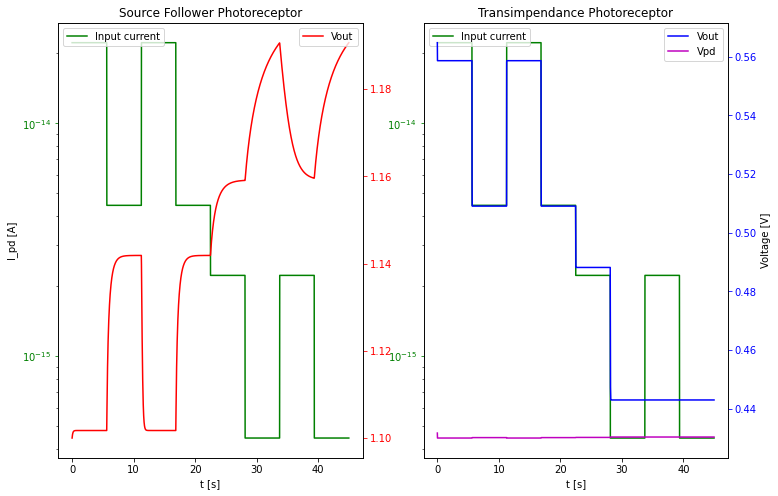
\includegraphics[width=0.75\linewidth]{Figures/photo_largesignal_response.png}
    \caption{Large signal transient photoreceptors responses}
    \label{fig:basalandcerebellum}
\end{figure}

\subsubsection{Small signal transient response}

\paragraph{Frequency response}

 TI photoreceptor is quicker in response to changes in photocurrent than the SF photoreceptor (and also noisier). 
 
In the simulation, we found a SF cutoff frequency of 289.31mHz and a TI cutoff frequency of 74.35Hz .

\begin{figure}[H]
    \centering
    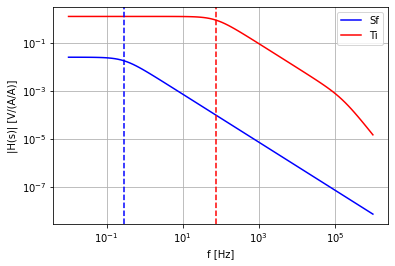
\includegraphics[width=0.75\linewidth]{Figures/photo_frequency.png}
    \caption{Bode plots of the photoreceptors}
    \label{fig:basalandcerebellum}
\end{figure}
 
To explain this numbers, we referred to the feedback of the TI photoreceptor, which increases tau and decreases the frequency. Since there are no peaks in the frequency response of the bode plot, the TI circuit moves slowly toward equilibrium (overdamped) at this $I_b$ and $I_{pd}$ .

\paragraph{Root locus plot}

The pole of the SF photoreceptor is defined as the frequency for which the value of the denominator of its transfer function becomes zero (as I like to say the poles define the undefined). 

The SF photoreceptor has a single pole and it moves farther away from the origin, as the photocurrent increases.  

On the other hand, the TI photoreceptor has two poles, because of the quadratic demoninator $D(s)$ of $H(s)$. To study them and plot their locations on a complex plane, we need what are called root locus plots. 

Root locus plots is a graphical analysis method used in control theory and stability theory. They examine how the roots of a system change with variation of a certain system parameter (in our case we will increase the amplfier bias current $I_b$).

The quality factor Q exists these poles. 

\begin{figure}[H]
    \centering
    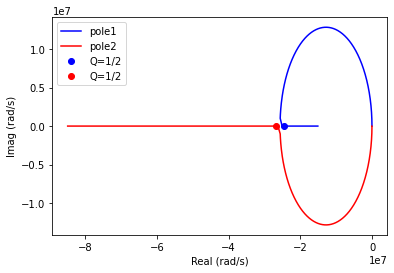
\includegraphics[width=0.75\linewidth]{Figures/photo_TIpoles.png}
    \caption{Poles of the transimpedance photoreceptor}
    \label{fig:basalandcerebellum}
\end{figure}

In the exactly critically-damped condition, the quality factor Q equals 0.5 . This means that at around $Q=0.5$, the voltage output of the TI photoreceptor returns as quickly as possible to its equilibrium position without oscillating back and forth.

\paragraph{Experiment}

From the conditions we defined above, we can experiment the small signal transient input photocurrent. 

We define a small signal transient input photocurrent with the following step size. 

\begin{figure}[H]
    \centering
    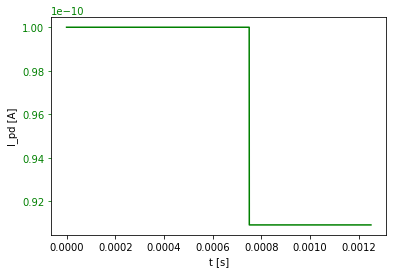
\includegraphics[width=0.75\linewidth]{Figures/photo_small.png}
    \caption{Small signal transient input photocurrent for TI photoreceptor}
    \label{fig:basalandcerebellum}
\end{figure}

With a quality factor of about 1/2, the TI photoreceptor biais current smooth the small signal transient input photocurrent. Doubling Q, let the curve approach more closely the input.

\begin{figure}[H]
    \centering
    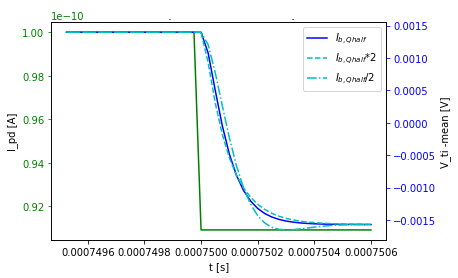
\includegraphics[width=0.75\linewidth]{Figures/photo_varyingQ.png}
    \caption{Small signal transient input photocurrent for TI photoreceptor, Q ~ 0.5}
    \label{fig:basalandcerebellum}
\end{figure}

We found the theoretical maximum Q at 8.95, using a bias current of around 4e-10A. However in such circumstances, the photoreceptor output has a ringing behavior. Apparently the the poles of the transfer function are not purely real.

\begin{figure}[H]
    \centering
    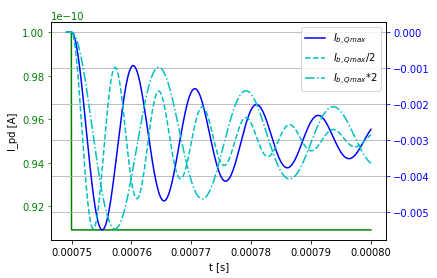
\includegraphics[width=0.75\linewidth]{Figures/photo_ringing.png}
    \caption{Small signal transient input photocurrent for TI photoreceptor, Q max}
    \label{fig:basalandcerebellum}
\end{figure}
